% main.tex -- arXiv paper source
% Build locally with ./build.sh (Tectonic). arXiv recompiles this source with pdfLaTeX
% (TeX Live 2025), so keep the preamble pdfLaTeX-compatible: no fontspec, no \pdfoutput,
% no raw Unicode symbols in the text.
\documentclass[11pt]{article}

% Fonts and encoding
\usepackage[utf8]{inputenc}
\usepackage[T1]{fontenc}
\usepackage{lmodern}
\usepackage{textcomp}
\usepackage{microtype}

% Math, figures, tables, lists, code
\usepackage{amsmath,amssymb,amsfonts}
\usepackage{graphicx}
\usepackage{booktabs}
\usepackage{array}
\usepackage{tabularx}
\usepackage{multirow}
\usepackage{xcolor}
\usepackage{caption}
\usepackage{subcaption}
\usepackage{enumitem}
\usepackage{listings}
\usepackage{tikz}
\usetikzlibrary{arrows.meta,positioning,shapes.geometric,fit,calc}
\usepackage[hyphens]{url}
\usepackage[hidelinks]{hyperref}

% Page geometry
\usepackage[margin=1in]{geometry}

% Allow slight stretch to avoid overfull boxes from long compound terms and URLs
\setlength{\emergencystretch}{2em}

% Table column types that wrap text: L{3cm} left-aligned, C{2cm} centered
\newcolumntype{L}[1]{>{\raggedright\arraybackslash}p{#1}}
\newcolumntype{C}[1]{>{\centering\arraybackslash}p{#1}}

% Code listing style (add language=Python etc. per listing)
\lstdefinestyle{paper}{
  basicstyle=\footnotesize\ttfamily,
  breaklines=true,
  frame=single,
  backgroundcolor=\color{gray!8},
  columns=flexible,
  keepspaces=true,
  showstringspaces=false,
  numbers=left,
  numberstyle=\tiny\color{gray},
  captionpos=b,
}
\lstset{style=paper}

% Paper version: printed under the title and used by ./build.sh release
\newcommand{\paperversion}{0.01}

% Title and authors
\title{From Researcher to Orchestrator: Attention-Bounded Supervision of AI Agent Teams in Engineering Research}

\author{
    Dan McCreary \\
    Independent Researcher, Minnesota, USA \\
    \small\url{https://www.linkedin.com/in/danmccreary/} \\
    \small ORCID: \href{https://orcid.org/0009-0009-3542-8828}{0009-0009-3542-8828}
}

\date{Version \paperversion \\ \today}

\begin{document}

\maketitle

% Abstract (write it last)
\begin{abstract}
Researchers in electrical and computer engineering increasingly delegate literature
search, coding, data analysis and drafting to AI agents, yet practices for supervising
several agents at once lag behind adoption, and the researcher remains accountable for
every claim. Existing multi-agent frameworks and levels-of-automation models do not tell a
researcher how much autonomy to grant a task, how work should pass between agents, or how
many agents one person can supervise. This paper presents an orchestration framework that
answers these questions. Each task's autonomy level is set from three properties of its
effects (reversibility, reach and verifiability) by a rule that is complete and
monotone. Work passes between agents as version-controlled files that no agent may mark
as accepted when it produced them, and every reported number must name the computation
that produced it. A review-load model bounds team size by the researcher's daily
attention and shows that the ratio of planning to execution agents follows from their
review costs rather than being fixed. We apply the framework to an illustrative
analog-to-digital converter characterization task and to two AI-assisted publication
projects, a 20-chapter textbook and an arXiv paper, whose logs and repositories record 13
defects. Mechanical checks caught every defect for which one existed, errors of meaning
were caught only when someone recomputed or read the work, and a quality score that no
computation had produced escaped every control and was published. The results suggest
measuring review load and escaped defects before enlarging an agent team.
\end{abstract}

\noindent\textbf{Keywords:} AI agents, human supervisory control, levels of autonomy,
multi-agent systems, research workflows, verification, reproducibility, electrical
engineering


% Main content sections -- one file per section, in reading order
\section{Introduction}
\label{sec:intro}

Large language model (LLM) agents now carry out multi-step research tasks rather than
answering single questions. An agent interleaves reasoning with tool calls---searching,
reading files, running code---and observes the results before choosing its next
action~\cite{yao2023react,wang2024survey,xi2025rise}. Researchers have adopted these tools
quickly. In a 2025 survey of 2,430 researchers, 84\% reported using AI tools, up from
57\% a year earlier~\cite{wiley2025explanaitions}; earlier surveys and corpus studies
found the same trend in attitudes and in the text of published
papers~\cite{vannoorden2023ai,liang2024mapping}. Electrical and computer engineering is
no exception: LLMs already generate and debug register-transfer-level hardware
descriptions~\cite{thakur2023benchmarking,blocklove2023chipchat,liu2023verilogeval}, and
domain-adapted models assist chip-design engineers~\cite{liu2023chipnemo}.

Practice has not kept pace with adoption. In the same survey, 57\% of researchers named a
lack of guidelines and training as a barrier, and the share concerned about inaccurate
output rose from 51\% to 64\%~\cite{wiley2025explanaitions}. The concern is well
founded. Language models produce fluent but false statements~\cite{ji2023survey};
in one study, 55\% of the bibliographic citations produced by GPT-3.5 and 18\% of those
produced by GPT-4 were fabricated~\cite{walters2023fabrication}. Models tend to agree with
their users~\cite{sharma2023sycophancy}, coding agents can satisfy tests by exploiting
them instead of meeting the specification~\cite{zhong2025impossiblebench}, and an
analysis of more than 1,600 execution traces from seven multi-agent frameworks
identified 14 distinct failure modes~\cite{cemri2025multiagent}. Meanwhile, venues and
funders agree that an AI tool cannot be an author and that the human authors take full
responsibility for everything a paper
contains~\cite{arxiv2025genai,thorp2023chatgpt,nature2023tools,ec2025living}. The
researcher therefore remains accountable for work that is increasingly performed by
systems that act on their own.

Two bodies of work bracket this problem without solving it. Multi-agent frameworks and
``AI scientist'' systems coordinate agents with each other and push toward greater
autonomy~\cite{wu2023autogen,hong2023metagpt,qian2024chatdev,lu2024aiscientist,schmidgall2025agentlab};
the human, where present, is an approver of last resort, and work passes between agents
as conversation. Research on levels of automation and human supervisory control models
exactly the quantity that matters---how much a human operator can oversee---but it was
developed for operators of vehicles and robots, not for agents that deliver asynchronous
documents and code whose cost lies in
verification~\cite{sheridan1978human,parasuraman2000model,crandall2005validating,cummings2008predicting}.
Recent proposals grade the autonomy of AI agents by the role the user
plays~\cite{feng2025levels}, but they do not say how to assign a level to a given task or
how many agents a single person can responsibly supervise. What is missing is an
operational framework that tells a researcher three things: how much autonomy to grant
each task, how work should pass between agents so that it stays reviewable, and how
large a team their attention can support.

This paper develops such a framework and examines it against three cases. It condenses
and formalizes the central argument of the author's open textbook \textit{AI for EE
Research}~\cite{mccreary2026aiforee}: that the researcher's role shifts from performing
each task to \textit{orchestrating} a team of planning and execution agents, while
remaining accountable for what is claimed. Our thesis is that the binding constraint on
such a team is not the number of agents that can be launched but the researcher's review
attention, and that a framework which makes this constraint explicit also places checks
where the defects that matter occur.

This paper makes the following contributions:
\begin{enumerate}[leftmargin=*]
  \item \textbf{An orchestration framework for research agent teams}
        (Section~\ref{sec:framework}): defined roles, a four-level autonomy scale, and an
        assignment rule that sets each task's level from three properties of its
        effects---reversibility, reach and verifiability. We show that the rule is
        complete and monotone.
  \item \textbf{A file-based handoff protocol} with five statuses and a
        separation-of-acceptance invariant, under which no agent may accept its own
        output, together with a provenance rule for reported numbers that the case
        analysis showed to be necessary.
  \item \textbf{An attention-budget model of review load} that yields the span of control
        of one researcher, shows that the ratio of planning to execution agents follows
        from their review costs rather than being a constant, and relates both to the
        fan-out models of human supervisory control.
  \item \textbf{A three-case evaluation}: an illustrative characterization task from
        analog-to-digital converter (ADC) research, and two real AI-assisted publication
        projects---a 20-chapter textbook and an arXiv paper---whose logs and
        repositories record 13 defects, analyzed by the control that caught each one or
        failed to.
\end{enumerate}

Section~\ref{sec:related} reviews related work on agents, automated science, LLMs in
hardware design, supervisory control and verification. Section~\ref{sec:framework}
presents the framework. Section~\ref{sec:cases} states the research questions and the
case-study method and reports the three cases and the cross-case analysis.
Section~\ref{sec:discussion} discusses implications and limitations, and
Section~\ref{sec:conclusion} concludes with directions for measurement.

\section{Background and Related Work}
\label{sec:related}

Five strands of prior work bear on how a researcher should supervise a team of agents.
Each subsection summarizes one strand and states how this paper builds on it or departs
from it. Table~\ref{tab:related} summarizes the comparison.

\subsection{LLM agents and multi-agent frameworks}
\label{sec:rw-agents}

An LLM agent couples a language model with tools and a loop: it decides on an action,
calls a tool, observes the result and decides again~\cite{yao2023react}. Surveys
organize the design space of single agents, for example into profile, memory, planning
and action modules~\cite{wang2024survey}, and of societies of cooperating
agents~\cite{xi2025rise}. Multi-agent frameworks compose several such
agents. AutoGen builds applications from conversable agents that exchange
messages~\cite{wu2023autogen}; MetaGPT encodes standardized operating procedures and
assigns software-company roles to agents~\cite{hong2023metagpt}; ChatDev organizes
role-playing agents into chat-based development phases~\cite{qian2024chatdev}; CAMEL
studies cooperation between role-playing agents~\cite{li2023camel}; and HuggingGPT uses
one model as a controller that plans tasks and dispatches them to specialist
models~\cite{shen2023hugginggpt}. Separating planning from execution also helps at the
level of a single prompt~\cite{wang2023planandsolve}. Practitioner reports distinguish
\textit{workflows}, whose steps are fixed in code, from \textit{agents}, which direct
their own tool use, and recommend an orchestrator--worker pattern for tasks that cannot
be decomposed in advance~\cite{schluntz2024building}; a production research system built
this way used roughly fifteen times the tokens of a chat interaction~\cite{hadfield2025multiagent}.
Agent behavior is increasingly configured through plain files---project instruction files
such as \texttt{AGENTS.md}~\cite{agentsmd2025} and packaged \textit{skills} with a
\texttt{SKILL.md} entry point~\cite{agentskills2025spec}---and coding agents are evaluated
on real repository tasks~\cite{jimenez2023swebench}. The failures of multi-agent systems
cluster into system-design issues, inter-agent misalignment and inadequate task
verification~\cite{cemri2025multiagent}.

This paper adopts the planner--executor and orchestrator--worker patterns and the use of
plain files as configuration. It departs from the frameworks above in two respects. The
orchestrator is the human researcher, whose review time is treated as the scarce
resource, and work passes between agents as versioned files with an explicit status,
not as conversation, so that every handoff can be read, diffed and accepted or rejected.

\subsection{AI systems that automate science}
\label{sec:rw-science}

A parallel line of work aims to automate research itself. The AI Scientist generates
ideas, runs experiments, writes papers and reviews them automatically~\cite{lu2024aiscientist}.
Coscientist designs, plans and executes chemistry experiments through laboratory
automation~\cite{boiko2023autonomous}, and ChemCrow augments a model with expert chemistry
tools~\cite{bran2024chemcrow}. Agent Laboratory takes a human-provided idea through
literature review, experimentation and report writing~\cite{schmidgall2025agentlab}, and
Co-Scientist uses a multi-agent system to generate and refine
hypotheses~\cite{gottweis2025coscientist}. Critics warn that such tools can produce
illusions of understanding, in which scientists believe they understand more than they
do, and can narrow the questions a field asks~\cite{messeri2024illusions}. Others argue
that risk to people grows with an agent's autonomy and that fully autonomous agents should
not be built~\cite{mitchell2025fully}.

Our framework sits at the opposite end of the autonomy range. It keeps the framing of the
question, the choice between approaches and the acceptance of every reported claim with
the researcher, consistent with the accountability required by venues and
funders~\cite{arxiv2025genai,thorp2023chatgpt,nature2023tools,ec2025living}. It also
starts from a constraint specific to engineering: much of the evidence is a physical
measurement, which an agent can analyze but must never be allowed to stand in for.

\subsection{LLMs in hardware design}
\label{sec:rw-eda}

In electrical and computer engineering, work on LLMs has concentrated on design
artifacts. Benchmarks measure the quality of generated Verilog~\cite{thakur2023benchmarking,liu2023verilogeval};
conversational design studies show an engineer and a model co-designing hardware
through dialogue~\cite{blocklove2023chipchat}; and domain-adapted models support
engineering assistance, script generation and bug summarization in chip
design~\cite{liu2023chipnemo}. These studies ask how capable a model is on a design task.
This paper asks a complementary question: given capable models, how should the
researcher who uses them divide, supervise and verify the work of several at once.

\subsection{Levels of automation and human supervisory control}
\label{sec:rw-loa}

Sheridan and Verplank's ten-level scale for supervisory control of teleoperators is the
origin of most \textit{levels of automation}~\cite{sheridan1978human}. Parasuraman,
Sheridan and Wickens separated the type of function automated (information acquisition,
analysis, decision and action) from the level of automation, and proposed that the level
be chosen by evaluating human-performance consequences together with automation
reliability and the costs of decision and action outcomes~\cite{parasuraman2000model}.
Mixed-initiative interfaces weigh the expected value of acting autonomously against that
of asking the user~\cite{horvitz1999principles}; design guidelines for human--AI
interaction~\cite{amershi2019guidelines} and human-centered AI~\cite{shneiderman2020hcai}
argue that high automation and high human control can coexist. For AI agents, Feng,
McDonald and Zhang define five levels by the role the user plays---operator,
collaborator, consultant, approver and observer---and propose autonomy certificates;
they treat autonomy as a design decision separate from capability~\cite{feng2025levels}.
Visibility measures such as agent identifiers, real-time monitoring and activity logs
make agents' actions inspectable after the fact~\cite{chan2024visibility}. Our own
earlier work described advocate agents that act on a person's behalf using explicit,
machine-readable preferences~\cite{ketter2008advocate}.

A second tradition asks how many semi-autonomous systems one person can supervise.
Crandall et al.\ characterized each robot by its \textit{neglect tolerance}---how long
it can be left unattended before its performance degrades---and by the interaction time
needed to restore it, and used the two to estimate the maximum number of robots one
person can manage, a quantity often called \textit{fan-out}~\cite{crandall2005validating}.
Cummings and Mitchell added the wait times that accrue from cognitive reorientation,
from vehicles queueing for the operator, and from lost situation awareness; including
them lowered predicted operator capacity by up to 67\% in their
simulation~\cite{cummings2008predicting}.

We borrow two ideas from this strand: that the level of automation should follow from the
consequences of the action, and that a supervisor's capacity can be computed from the
attention each subordinate system demands. We depart from it in the object being
supervised. A research agent does not need continuous control; it delivers discrete
artifacts---a reading list, a script, a table, a paragraph---whose cost to the human is
the time needed to verify them. Our assignment rule (Section~\ref{sec:autonomy}) makes the
consequence criterion concrete for research tasks, and our review-load model
(Section~\ref{sec:attention}) is a fan-out model for asynchronous artifacts.

\subsection{Automation bias, LLM failure modes and verification}
\label{sec:rw-verification}

People supervising automation tend toward complacency and automation bias: they monitor
less and accept automated recommendations with less scrutiny, especially when the
automation is usually right~\cite{parasuraman2010complacency,goddard2012automation}. LLM
output adds failure modes of its own: hallucination~\cite{ji2023survey}, fabricated and
erroneous citations~\cite{walters2023fabrication}, sycophancy~\cite{sharma2023sycophancy},
degraded use of information in the middle of long contexts~\cite{liu2024lost},
susceptibility to instructions injected through retrieved content~\cite{greshake2023injection},
and, for coding agents, a propensity to exploit test cases~\cite{zhong2025impossiblebench}.
Using one model to judge another scales review but brings biases of its
own~\cite{zheng2023judging}. Against these, scientific computing has long recommended
version control, scripted analysis, recorded provenance and tests~\cite{sandve2013ten,wilson2014best,wilson2017good},
and computational science distinguishes \textit{verification} (solving the equations
right) from \textit{validation} (solving the right equations)~\cite{oberkampf2010vv}.

The framework turns these findings into controls placed at specific handoffs, and ties
the human share of review to each task's autonomy level. Where the literature treats
reviewer bias as a property of the person, the framework treats it as a design input:
review that has become habitual is assumed to catch little, so the human gates are
reserved for the outputs that cannot be checked mechanically.

\begin{table}[htbp]
  \centering
  \caption{How this paper relates to the main strands of prior work. ``Capacity'' asks
  whether the approach models how much a single human can supervise.}
  \label{tab:related}
  \small
  \begin{tabular}{L{3.0cm}L{2.5cm}L{2.7cm}L{2.5cm}L{2.6cm}}
    \toprule
    Approach & Unit supervised & Human role & Autonomy set by & Capacity \\
    \midrule
    Multi-agent LLM frameworks~\cite{wu2023autogen,hong2023metagpt,qian2024chatdev} &
      Agent conversation & Optional participant or approver & System configuration &
      Not a design variable \\
    Automated-science systems~\cite{lu2024aiscientist,schmidgall2025agentlab,gottweis2025coscientist} &
      Research pipeline & Supplies idea; reads output & High by design &
      Not a design variable \\
    Supervisory control~\cite{sheridan1978human,parasuraman2000model,crandall2005validating} &
      Vehicle or robot & Supervisor & Level scale; consequences & Fan-out from neglect and interaction time \\
    Agent autonomy levels~\cite{feng2025levels} &
      Agent & One of five user roles & Design decision; certificates & Not modelled \\
    \textbf{This paper} &
      Research task and its artifact & Orchestrator; sole acceptor of claims &
      Reversibility, reach, verifiability & Daily review-attention budget \\
    \bottomrule
  \end{tabular}
\end{table}

\section{The Orchestration Framework}
\label{sec:framework}

The framework has four parts: a vocabulary of roles, a rule that sets each task's
autonomy, a protocol by which work passes between agents, and a model of the researcher's
review attention that bounds the size of the team. Figure~\ref{fig:overview} shows how
the parts fit together. The material condenses Chapters 1, 9, 10 and 17 of the source
textbook~\cite{mccreary2026aiforee}; the formal statements, the monotonicity result, the
derived planning-to-execution ratio, the sampling and escape terms of the attention model,
and the provenance rule are this paper's additions.

\begin{figure}[htbp]
  \centering
  % Figure: overview of the orchestration framework (Section 4).
\definecolor{oiblue}{HTML}{0072B2}
\definecolor{oiorange}{HTML}{E69F00}
\definecolor{oigreen}{HTML}{009E73}
\definecolor{oipurple}{HTML}{CC79A7}
\begin{tikzpicture}[
    font=\footnotesize,
    box/.style={draw, rounded corners=2pt, align=center, minimum height=11mm, inner sep=3pt},
    arrow/.style={-{Latex[length=2mm]}, thick},
    lab/.style={font=\scriptsize, align=center, fill=white, inner sep=1pt}]
  \node[box, fill=gray!12, text width=80mm] (R)
    {\textbf{Researcher (orchestrator)}\\question and acceptance criteria $\cdot$ gates\\
     acceptance of claims $\cdot$ daily review budget $B$};
  \node[box, fill=oigreen!10, text width=50mm, below=17mm of R] (W)
    {\textbf{Shared workspace} (version-controlled files)\\each artifact carries a status:\\
     \textsf{queued} $\rightarrow$ \textsf{running} $\rightarrow$ \textsf{needs-review}\\
     $\rightarrow$ \textsf{accepted} / \textsf{rejected}};
  \node[box, fill=oiblue!10, text width=25mm, left=17mm of W] (P)
    {\textbf{Planning agents}\\($n_p$): survey,\\decompose, specify};
  \node[box, fill=oiorange!15, text width=25mm, right=19mm of W] (E)
    {\textbf{Execution agents}\\($n_e$): code,\\analysis,\\figures, text};
  \node[box, fill=oipurple!12, text width=50mm, below=11mm of W] (C)
    {\textbf{Checks}: tests, validators, strict build, reviewer agent};
  \draw[arrow] (R.west) -| node[lab, pos=0.78]{question,\\constraints} (P.north);
  \draw[arrow] (P.east) -- node[lab, above=1pt]{plans,\\specs} (W.west);
  \draw[arrow] ([yshift=2.5mm]W.east) -- node[lab, above=1pt]{tasks} ([yshift=2.5mm]E.west);
  \draw[arrow] ([yshift=-2.5mm]E.west) -- node[lab, below=1pt]{artifacts,\\checks run} ([yshift=-2.5mm]W.east);
  \draw[arrow] ([xshift=-9mm]W.south) -- node[lab, left=1pt]{needs-review} ([xshift=-9mm]C.north);
  \draw[arrow] ([xshift=9mm]C.north) -- node[lab, right=1pt]{pass / defects} ([xshift=9mm]W.south);
  \draw[arrow, very thick, densely dashed] (W.north) -- node[lab, right=2pt]{gate: claims, irreversible\\or outward-bound actions} (R.south);
  \draw[arrow] (R.east) -| node[lab, pos=0.78]{approve\\level-1 steps} (E.north);
\end{tikzpicture}

  \caption{The orchestration framework. Planning agents turn the researcher's question
  into plans and specifications; execution agents turn specifications into artifacts.
  All work passes through a shared, version-controlled workspace in which each artifact
  carries a status. Scripts and reviewer agents check artifacts, but only the researcher
  accepts claims and approves irreversible or outward-bound actions. Note that the
  researcher's daily review budget $B$, not the number of agents, sets the team size.}
  \label{fig:overview}
\end{figure}

\subsection{Definitions}
\label{sec:definitions}

\begin{description}[leftmargin=1.2em,style=nextline]
  \item[Research workflow] The sequence of repeatable activities by which a research
    question becomes a validated, communicated result: literature search, problem
    framing, scientific coding, data analysis and manuscript preparation, chained so that
    the output of each is the input of the next.
  \item[Task and artifact] A task is a unit of delegated work with a stated input, a
    bounded scope, an inspectable output (the \textit{artifact}) and an acceptance check
    that can pass or fail without redoing the work.
  \item[Agent] A system that uses a language model to choose actions, invokes tools to
    take them, observes the results and repeats until a goal is met or it stops to
    ask~\cite{yao2023react}. An \textit{assistant} differs in that the human takes every
    action in the world.
  \item[Orchestrator] Whoever decides what is done, by which agent, in what order, with
    what checks, and what happens on failure. Here the orchestrator is the researcher,
    who may be helped by an agent that keeps the task queue and drafts status reports but
    remains accountable for the result.
  \item[Check, gate and acceptance] A \textit{check} examines an artifact against its
    acceptance criteria; it may be mechanical (a test, a validator, a strict build) or
    performed by a reviewer agent. A \textit{gate} is a check at which the researcher
    must approve before work continues. \textit{Acceptance} is the decision that an
    artifact meets its criteria and may be used downstream.
\end{description}

\subsection{Roles}
\label{sec:roles}

Each agent holds one role, written once as a specification file and reused. One role
per agent has the same benefits as single-purpose software modules: a short instruction
set, a checkable output and failures that localize. Table~\ref{tab:roles} lists the
roles. The two primary roles differ in the cost of their output. A planning agent
surveys, decomposes and specifies; its output is a document that is cheap to read and
cheap to discard. An execution agent writes code, runs analyses and prepares figures and
text; its output changes files and consumes compute, and each unit costs more attention
to check. The \textit{planner--executor pattern} makes the specification the handoff
between them, so that a plan can be corrected before anything is
executed~\cite{shen2023hugginggpt,wang2023planandsolve,schluntz2024building}.
A reviewer agent checks another agent's output against stated criteria; because model
judges share the biases of models~\cite{zheng2023judging}, it complements mechanical
checks and the researcher's sampling rather than replacing them. Each agent receives
only the context its role needs (\textit{context isolation}), which limits distraction
in long contexts~\cite{liu2024lost} and limits what an agent that reads untrusted
content can leak or be steered into~\cite{greshake2023injection}.

\begin{table}[htbp]
  \centering
  \caption{Agent roles with their usual artifact, default autonomy ceiling (levels
  defined in Table~\ref{tab:levels}) and the check applied before acceptance. Domain
  roles specialize a planning or execution role.}
  \label{tab:roles}
  \small
  \begin{tabular}{L{2.6cm}L{4.3cm}L{2.9cm}C{1.3cm}L{3.0cm}}
    \toprule
    Role & Purpose & Artifact & Level & Check \\
    \midrule
    Planning & Survey, decompose, specify & Plan, specification & 2--3 & Researcher reads plan \\
    Execution & Carry out a specified task & Files, results & 1--2 & Acceptance criteria, tests \\
    Reviewer & Check output against criteria & Defect list & 3 & Sample of its findings \\
    \midrule
    Literature & Search, triage, extract claims & Reading list with claim locations & 2 & Citation lookup \\
    Analysis & Run statistical and signal processing & Tables, plots & 2 & Known-answer tests \\
    Coding & Write and test code & Scripts, tests & 2 & Tests, diff review \\
    Writing & Draft prose from claims & Section drafts & 2 & Claim audit by researcher \\
    \bottomrule
  \end{tabular}
\end{table}

\subsection{Autonomy levels and the assignment rule}
\label{sec:autonomy}

Autonomy is the degree to which an agent acts without a human decision at each step.
The framework uses four levels (Table~\ref{tab:levels}). Following the principle that
automation should be chosen by the consequences of actions~\cite{parasuraman2000model},
the level is set from three Boolean properties of a task's \emph{effects}, not from
confidence in the model:
\begin{itemize}[leftmargin=*]
  \item \textit{Reach} $X(t)$: the result leaves the researcher's control---it is sent,
    published, written to a shared system or commits resources ($X=1$).
  \item \textit{Reversibility} $R(t)$: the effect can be undone, as a change to a
    version-controlled file can and a sent message cannot ($R=1$).
  \item \textit{Verifiability} $V(t)$: the result can be checked quickly and
    objectively, by a script or a short human inspection ($V=1$); a program with tests is
    verifiable, a paragraph of related work is not without reading the cited papers.
\end{itemize}

\begin{table}[htbp]
  \centering
  \caption{Autonomy levels. The level is a ceiling for the task; an agent operates at or
  below it, and only after evaluation shows that it performs the task reliably.}
  \label{tab:levels}
  \small
  \begin{tabular}{C{0.9cm}L{3.0cm}L{5.0cm}L{5.2cm}}
    \toprule
    Level & Name & The agent may & Typical use \\
    \midrule
    0 & Suggest only & Propose; the researcher performs the action & Outward-bound results that cannot be verified \\
    1 & Approve each step & Act after each action is approved & Irreversible, or outward-bound but verifiable \\
    2 & Act within a boundary & Act inside a defined scope; stop at gates & Local, reversible work whose quality needs a human read \\
    3 & Act and report & Act unattended; report afterwards & Local, reversible, mechanically verifiable work \\
    \bottomrule
  \end{tabular}
\end{table}

The assignment rule, shown as a decision tree in Figure~\ref{fig:autonomy}, maps the three
properties to a level:
\begin{equation}
  \lambda(t) =
  \begin{cases}
    0 & \text{if } X=1 \text{ and } V=0,\\
    1 & \text{if } X=1 \text{ and } V=1, \text{ or } X=0 \text{ and } R=0,\\
    2 & \text{if } X=0,\ R=1 \text{ and } V=0,\\
    3 & \text{if } X=0,\ R=1 \text{ and } V=1.
  \end{cases}
  \label{eq:rule}
\end{equation}

\begin{figure}[htbp]
  \centering
  % Figure: the autonomy assignment rule, Equation (1), as a decision tree read left to right
% (Section 4.3).
\definecolor{oiblue}{HTML}{0072B2}
\definecolor{oivermillion}{HTML}{D55E00}
\begin{tikzpicture}[
    font=\footnotesize,
    q/.style={draw, rounded corners=2pt, align=center, fill=gray!10, text width=25mm, minimum height=9mm, inner sep=2pt},
    leaf/.style={draw, align=center, text width=24mm, minimum height=8.5mm, inner sep=2pt},
    arrow/.style={-{Latex[length=2mm]}, thick},
    yes/.style={font=\scriptsize, fill=white, inner sep=1pt}]
  \node[q] (X) at (0, 0) {Result leaves your control? (reach $X$)};
  \node[q] (V1) at (3.9, 1.6) {Verifiable? ($V$)};
  \node[q] (Rv) at (3.9, -1.3) {Reversible? ($R$)};
  \node[leaf, fill=oivermillion!22] (L0) at (8.0, 2.3) {\textbf{Level 0}\\Suggest only};
  \node[leaf, fill=oivermillion!8] (L1a) at (8.0, 0.95) {\textbf{Level 1}\\Approve each step};
  \node[leaf, fill=oivermillion!8] (L1b) at (8.0, -0.4) {\textbf{Level 1}\\Approve each step};
  \node[q] (V2) at (8.0, -2.2) {Verifiable? ($V$)};
  \node[leaf, fill=oiblue!8] (L2) at (12.1, -1.55) {\textbf{Level 2}\\Act within boundary};
  \node[leaf, fill=oiblue!22] (L3) at (12.1, -2.85) {\textbf{Level 3}\\Act and report};
  \draw[arrow] (X.east) -- node[yes]{yes} (V1.west);
  \draw[arrow] (X.east) -- node[yes]{no} (Rv.west);
  \draw[arrow] (V1.east) -- node[yes]{no} (L0.west);
  \draw[arrow] (V1.east) -- node[yes]{yes} (L1a.west);
  \draw[arrow] (Rv.east) -- node[yes]{no} (L1b.west);
  \draw[arrow] (Rv.east) -- node[yes]{yes} (V2.west);
  \draw[arrow] (V2.east) -- node[yes]{no} (L2.west);
  \draw[arrow] (V2.east) -- node[yes]{yes} (L3.west);
\end{tikzpicture}

  \caption{The autonomy assignment rule of Equation~\eqref{eq:rule} as a decision tree.
  Reach is tested first because an outward-bound result cannot be recalled, whatever
  its other properties. Note that an irreversible local action receives level 1 even when
  it is verifiable, since a check after the fact cannot undo it.}
  \label{fig:autonomy}
\end{figure}

\paragraph{Proposition 1 (completeness and monotonicity).} \textit{The rule assigns
exactly one level to each of the eight combinations of $(X,R,V)$, and making a task safer
in any one property---$X$ from 1 to 0, $R$ from 0 to 1, or $V$ from 0 to 1---never lowers
its level.}

\textit{Proof.} The four cases partition the space: $X=1$ is split by $V$, and $X=0$ is
split by $R$ and then, for $R=1$, by $V$. For monotonicity, consider each property in
turn. Raising $V$ moves $(X{=}1)$ from 0 to 1, leaves $(X{=}0,R{=}0)$ at 1, and moves
$(X{=}0,R{=}1)$ from 2 to 3. Raising $R$ leaves $X=1$ tasks unchanged and moves $X=0$
tasks from 1 to 2 or 3. Lowering $X$ moves $(V{=}0)$ tasks from 0 to 1 or 2 and $(V{=}1)$
tasks from 1 to 1 or 3. No transition decreases the level. $\square$

Monotonicity matters in practice because the cheapest way to raise an agent's autonomy is
to change the task, not the model: writing outputs to a new file instead of overwriting
raw data makes an action reversible, and adding a known-answer test makes it verifiable.
The level is a \emph{ceiling}. An agent operates at $\min(\lambda(t), \ell_e)$, where
$\ell_e$ is the level its evaluation on representative tasks supports; the evaluation is
repeated whenever the model, tools or instructions change.

\subsection{Failure modes and controls}
\label{sec:failures}

Agents fail in recognizable ways, and each failure leaves a signature in a log.
Table~\ref{tab:failures} lists six modes with the mechanical defense the framework
prescribes for each; they correspond to the system-design and task-verification
failures observed in multi-agent traces~\cite{cemri2025multiagent} and to test
exploitation by coding agents~\cite{zhong2025impossiblebench}. Logging is therefore a
precondition of autonomy above level 1: for each step the log records the time, the
tool and its arguments, the files changed, the model and its settings, and the result,
as activity logging proposals for agents recommend~\cite{chan2024visibility}.

\begin{table}[htbp]
  \centering
  \caption{Agent failure modes, how each appears in a log, and the mechanical defense
  that removes the need to catch it by careful reading.}
  \label{tab:failures}
  \small
  \begin{tabular}{L{3.0cm}L{5.4cm}L{5.8cm}}
    \toprule
    Failure mode & Log signature & Mechanical defense \\
    \midrule
    Premature completion & ``Done'' reported with no check output & Require the check output in the handoff \\
    Hallucinated result & A reported number with no producing tool call & Provenance rule: trace every number to a call \\
    Scope drift & Edits to files outside the task & Path permissions; diff review \\
    Test weakening & Test files changed alongside failing code & Protect tests; review test diffs first \\
    Wrong arguments & Tool errors, or results from the wrong file & Read the first calls of a new workflow \\
    Runaway loop & The same call repeated without progress & Step, time and spending limits; repeat detector \\
    \bottomrule
  \end{tabular}
\end{table}

\subsection{Handoff protocol and provenance}
\label{sec:handoff}

Work passes between agents as files in a shared, version-controlled workspace. Each
agent writes to its own directory or branch, inputs are read-only, and merging is a
reviewed step. Every artifact carries a status from the set
$S=\{\textsf{queued},\textsf{running},\textsf{needs-review},\textsf{accepted},\textsf{rejected}\}$,
with transitions $\textsf{queued}\rightarrow\textsf{running}\rightarrow\textsf{needs-review}
\rightarrow\{\textsf{accepted},\textsf{rejected}\}$ and $\textsf{rejected}\rightarrow\textsf{queued}$.
The protocol imposes three invariants and one rule:
\begin{enumerate}[leftmargin=*,label=\textbf{I\arabic*}]
  \item \textit{Separation of acceptance.} For every artifact $a$,
    $\mathrm{acceptor}(a)\neq\mathrm{producer}(a)$: no agent sets \textsf{accepted} on its
    own output. A script, a reviewer agent or the researcher may.
  \item \textit{Level-bounded acceptors.} Artifacts of level-3 tasks may be accepted by a
    script; artifacts of level-0 and level-1 tasks are accepted only by the researcher.
  \item \textit{Claim gate.} Any artifact whose content becomes a reported
    claim---a number, a citation or a conclusion in a manuscript---is accepted only by the
    researcher, whatever the level of the task that produced it.
  \item[\textbf{P}] \textit{Provenance.} Every number that an agent reports as computed
    names the command or script and the input that produced it. A number without a
    producing call is treated as unverified and blocks acceptance.
\end{enumerate}
The provenance rule was added after the case analysis of Section~\ref{sec:cross-case}
showed a defect that no other control could catch. A handoff record that satisfies the
protocol fits in a few lines (Listing~1).

\begin{lstlisting}[caption={An illustrative handoff record for the ENOB analysis script of
Section~\ref{sec:case-a}, written as YAML at the top of the artifact.}]
task: T3-enob-script          # from the task queue
role: coding-agent            # producer
level: 3                      # ceiling from Eq. (1): local, reversible, verifiable
status: needs-review          # producer may not set "accepted" (I1)
inputs: [docs/procedure.md@a1c3f2, data/ideal-10bit.csv]
outputs: [scripts/enob.py]    # the only path it may write
acceptance:
  - known-answer: ideal 10-bit record gives SNDR 61.96 dB (+/- 0.05)
  - boundary: empty or wrong-length record raises an error
check_output: logs/T3-check.txt
numbers:                       # provenance rule P
  - {value: "61.96 dB", source: "logs/T3-check.txt:14"}
open_questions: [window choice for non-coherent records]
\end{lstlisting}

\subsection{Attention budget and span of control}
\label{sec:attention}

Let a team have $n_p$ planning and $n_e$ execution agents. An agent of class
$j\in\{p,e\}$ delivers $k_j$ artifacts per day; reading one takes the researcher $r_j$
minutes; the researcher reads a fraction $s_j\in(0,1]$ of them; and conflict resolution
and status reports take $c$ minutes a day. The daily review load is
\begin{equation}
  L = n_p k_p r_p s_p + n_e k_e r_e s_e + c ,
  \label{eq:load}
\end{equation}
and the team is feasible when $L\leq B$, the researcher's daily attention budget. For a
team of one class the \textit{span of control} is
\begin{equation}
  n_j^{\max} = \left\lfloor \frac{B-c}{k_j\, r_j\, s_j} \right\rfloor .
  \label{eq:span}
\end{equation}
Equation~\eqref{eq:span} plays the role of fan-out in supervisory
control~\cite{crandall2005validating,cummings2008predicting}: an agent that delivers an
artifact every $1/k_j$ days and needs $r_j s_j$ minutes of attention for each can be
neglected for the rest of the time. The difference is that the attention is spent on
verification after the fact rather than on control during the task.

The book's worked example uses illustrative values: $n_p=20$ and $n_e=10$, one artifact
per agent per day, $r_p=6$ and $r_e=15$ minutes, $s_p=s_e=1$ and $c=30$ minutes. Then
$L=120+150+30=300$ minutes. With a budget of four hours ($B=240$), the team is infeasible;
reading half of the planning artifacts ($s_p=0.5$) gives $L=60+150+30=240$ and restores
feasibility. Figure~\ref{fig:load} shows the load as the team grows under three review
regimes.

\begin{figure}[htbp]
  \centering
  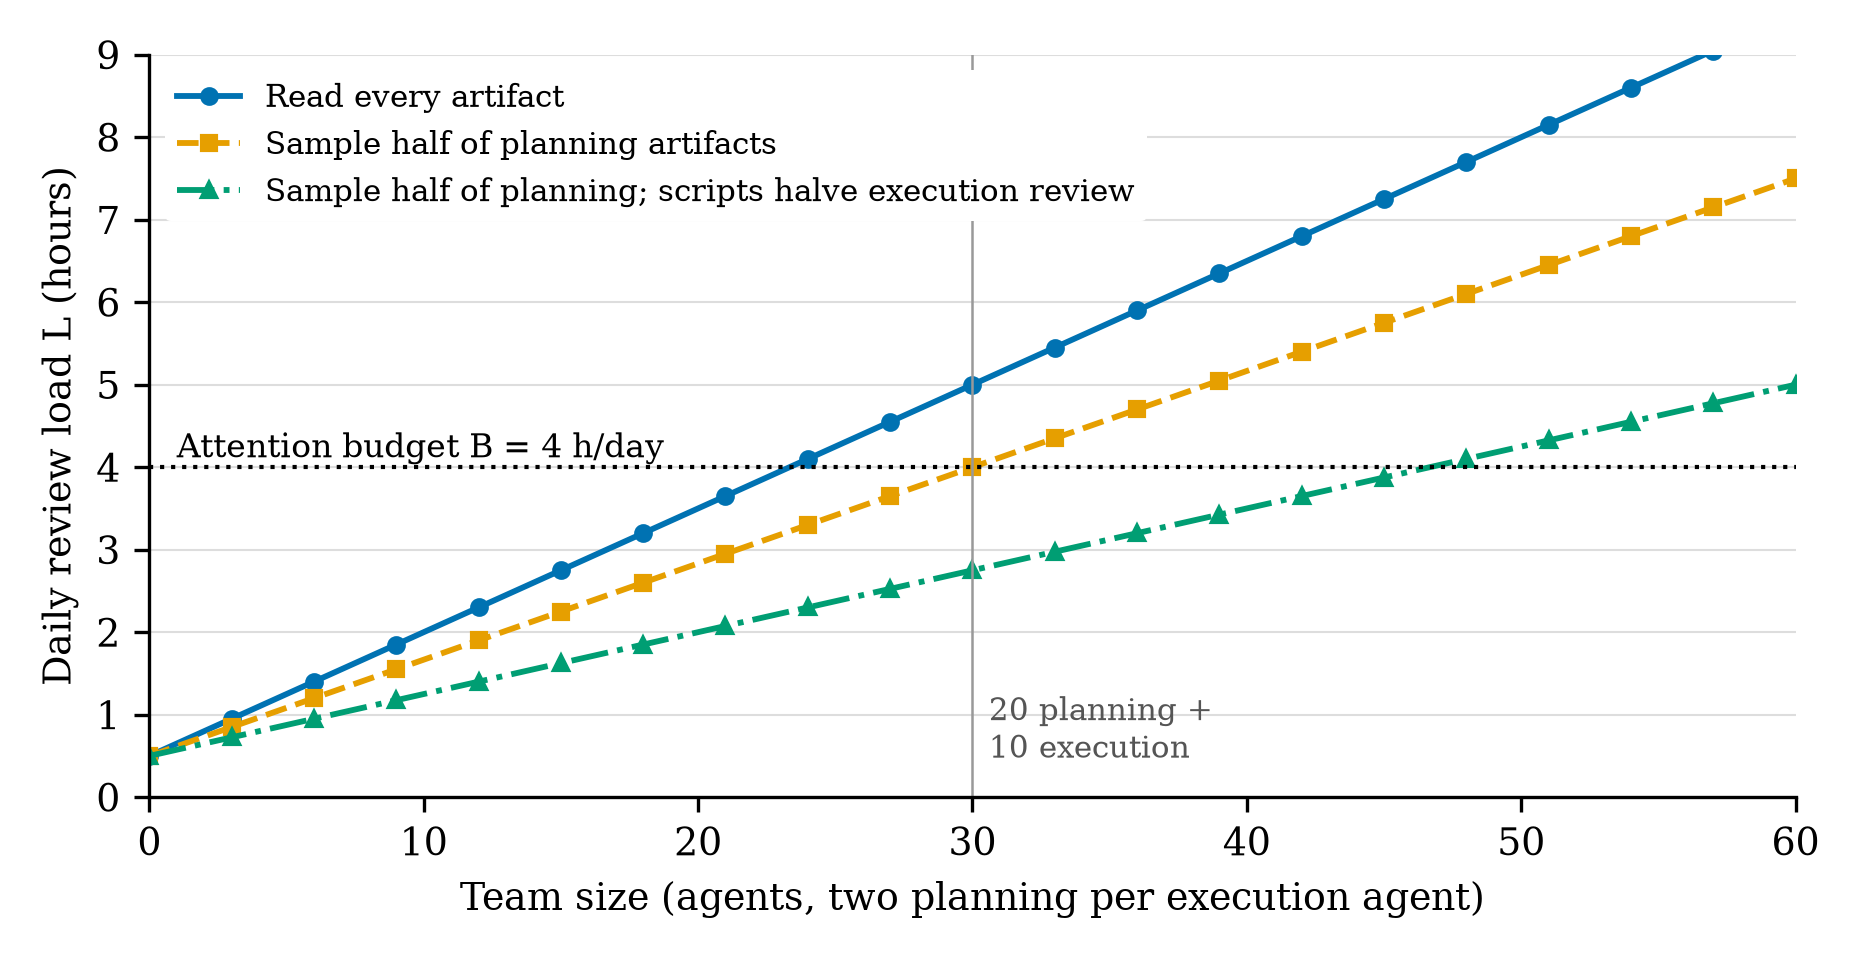
\includegraphics[width=0.85\textwidth]{figures/review-load.png}
  \caption{Daily review load $L$ (Equation~\ref{eq:load}) against team size for a team
  with two planning agents per execution agent, under three review regimes, with a
  four-hour attention budget. Parameters are the illustrative values of
  Section~\ref{sec:attention}, not measurements. Note that sampling planning output and
  replacing part of execution review with scripted checks each widen the span of
  control more than any change in the number of agents can.}
  \label{fig:load}
\end{figure}

\paragraph{The planning-to-execution ratio is derived, not fixed.} Suppose the researcher
gives a share $\beta$ of the net budget $B-c$ to reviewing plans. Applying
Equation~\eqref{eq:load} to each class gives
\begin{equation}
  \frac{n_p}{n_e} = \frac{\beta}{1-\beta}\cdot\frac{k_e\, r_e\, s_e}{k_p\, r_p\, s_p}.
  \label{eq:ratio}
\end{equation}
With the illustrative costs and an equal split ($\beta=0.5$) the ratio is $15/6=2.5$; the
book's 20:10 team corresponds to $\beta=120/270\approx0.44$. The ratio is therefore a
consequence of the relative cost of reviewing plans and executions. A known-answer test
that halves $r_e$ doubles the number of execution agents the same budget supports.

\paragraph{Sampling trades load for escaped defects.} Let an artifact of class $j$
contain a consequential defect with probability $q_j$, let mechanical checks detect it
with probability $a_j$, and let the researcher detect it with probability $h_j$ when the
artifact is read. The expected number of defects per day that pass review undetected is
\begin{equation}
  E = \sum_{j\in\{p,e\}} n_j\, k_j\, q_j\,(1-a_j)\,(1-s_j h_j).
  \label{eq:escape}
\end{equation}
Lowering $s_j$ reduces $L$ linearly but raises $E$; raising $a_j$ lowers $E$ without any
cost in $L$. Automation bias lowers $h_j$ as the researcher grows used to correct
output~\cite{parasuraman2010complacency}, so the framework prefers mechanical checks to
reduced sampling, reserves sampling for reversible planning output, and requires
reviewers to state an expected value or check a random sample rather than approve by
habit. $E$ is observable as the number of defects found after acceptance, and together
with $L$ it is the quantity to measure before a team is enlarged.

\paragraph{Checks at handoffs dominate improvements to single stages.} For a chain of $m$
stages in which stage $i$ introduces a consequential defect with probability $p_i$ and
the check at its handoff catches it with probability $d_i$, the probability that the
final result is free of such defects is
\begin{equation}
  P_{\mathrm{clean}} = \prod_{i=1}^{m}\bigl(1 - p_i(1-d_i)\bigr).
  \label{eq:pipeline}
\end{equation}
With five stages and $p_i=0.1$ (illustrative), $P_{\mathrm{clean}}=0.9^5\approx0.59$ with
no checks. Making one stage almost perfect ($p=0.01$) raises it only to about $0.65$,
whereas a check catching 80\% of defects at every handoff raises it to
$0.98^5\approx0.90$.

\paragraph{Dependencies bound what parallelism can buy.} The makespan of a set of tasks
cannot be shorter than the longest chain of dependent tasks, the critical
path~\cite{kelley1959critical}, however many agents are available, and each added agent
adds handoffs and potential conflicts~\cite{brooks1995mythical}. A team should therefore
grow one role at a time, and stop when an added agent adds more review than it removes
work.

\subsection{Design rationale and rejected alternatives}
\label{sec:rationale}

Five design decisions distinguish the framework, each taken against a named
alternative.
\begin{enumerate}[leftmargin=*]
  \item \textit{Autonomy from task effects, not model capability.} Capability-based
    levels change with every model release and say nothing about whether a result can be
    recalled. Role-based levels~\cite{feng2025levels} describe the interaction but give no
    rule for a task; the rule of Equation~\eqref{eq:rule} supplies one and is compatible
    with them (roughly, level 0 corresponds to the user as operator, level 1 to the user
    as approver and level 3 to the user as observer).
  \item \textit{Files, not conversations, as handoffs.} Conversational
    coordination~\cite{wu2023autogen,qian2024chatdev} is flexible, but a conversation is
    hard to diff, review or resume a month later. Files in version control give every
    handoff an author, a timestamp and a reversible history, at the cost of more
    up-front structure.
  \item \textit{A human orchestrator, not an autonomous one.} Fully automated research
    pipelines~\cite{lu2024aiscientist,schmidgall2025agentlab} remove the bottleneck this
    paper models, but they also remove the accountable party that venues
    require~\cite{arxiv2025genai,thorp2023chatgpt}, and they cannot produce physical
    measurements. An orchestrating agent may keep the queue; it may not accept claims.
  \item \textit{Reviewer agents as complements.} A reviewer agent scales review but
    shares the failure modes of the models it
    reviews~\cite{zheng2023judging,sharma2023sycophancy}; it is used to decide where the
    researcher looks, not what is true.
  \item \textit{Risk-weighted sampling instead of reading everything.} Reading every
    artifact is infeasible beyond a small team (Figure~\ref{fig:load}) and invites
    habitual approval~\cite{goddard2012automation}. The framework samples only reversible
    planning output and keeps full review for claims and irreversible actions.
\end{enumerate}

\section{Case-Study Evaluation}
\label{sec:cases}

\subsection{Research questions and method}
\label{sec:method}

We examine the framework against three cases to answer three questions.
\begin{description}[leftmargin=1.2em,style=nextline]
  \item[RQ1 (coverage)] Can each element of the framework---roles, autonomy levels,
    handoff protocol and review budget---be identified in, or applied to, a concrete
    AI-assisted research or publication workflow?
  \item[RQ2 (detection)] Which defects arose in those workflows, and which control
    detected each one?
  \item[RQ3 (escape)] Which defects escaped the controls, and what change to the
    framework do they imply?
\end{description}

The study follows a multiple-case design~\cite{yin2018case}. Case~A applies the framework
to an electrical-engineering characterization task; it is \emph{illustrative}, and all
of its values come from the worked examples of the source book rather than from a
measured project. Cases~B and~C are real projects of the author, chosen because their
complete records are available: repositories under version control, session logs written
during the work, and public outputs. For Case~B the data are the project instruction
file, four session logs, twenty per-chapter timestamp files, the learning-graph data and
reports, the status field of each of the 50 simulation pages, and the commit history up to
commit \texttt{8732aa0} (34 commits between 15 and 22 October 2026). For Case~C the data are the paper's folder in
its repository (readme, status file, section files and figure script), its commit
history (23 commits between 17 October and 24 November 2025) and the posted
preprint~\cite{lockhart2025microsims}. Every defect recorded in these sources was coded
by the stage at which it entered, its failure mode (Table~\ref{tab:failures}, or
\textit{specification error} for a defect in a plan), the control that detected it, and
the type of that control: mechanical, agent, independent calculation, human gate, or
none. The author performed the coding alone; Section~\ref{sec:limitations} discusses the
consequences.

\subsection{Case A: characterizing an ADC (illustrative)}
\label{sec:case-a}

\paragraph{Context.} A doctoral student designs a low-power successive-approximation-register
(SAR) ADC for battery-powered sensor nodes and must show whether it meets a resolution target.
The research question carries its own stopping rule: \textit{can a 10-bit
charge-redistribution SAR ADC in a 65~nm process reach an effective number of bits
(ENOB) of at least 9.5 at 1~MS/s while drawing less than 50~$\mu$W?} ENOB relates the
measured signal-to-noise-and-distortion ratio (SNDR) to an equivalent ideal
resolution~\cite{ieee1241},
\begin{equation}
  \mathrm{ENOB} = \frac{\mathrm{SNDR}_{\mathrm{dB}} - 1.76}{6.02},
  \label{eq:enob}
\end{equation}
so that an ideal $N$-bit quantizer driven by a full-scale sine wave has
$\mathrm{SNDR}=6.02N+1.76$~dB, or 61.96~dB for $N=10$.

\paragraph{Applying the framework.} The goal decomposes into nine tasks with the
dependencies and illustrative durations of Figure~\ref{fig:adc}. Table~\ref{tab:case-a}
applies the assignment rule of Equation~\eqref{eq:rule} to each. Three features of the
result are worth noting. First, the ENOB script reaches level~3 only because it has a
\emph{known-answer test}: fed the output of an ideal 10-bit quantizer, it must return
61.96~dB, and a script that returns 58 or 66~dB is wrong whatever else it appears to do.
The test suite itself stays at level~2: no quick check shows that a test suite is
adequate, and coding agents have been observed to modify or exploit tests rather than
meet the specification~\cite{zhong2025impossiblebench}. Second, the one irreversible
action an analysis agent might propose---overwriting raw measurement files with cleaned
versions---is assigned level~1; redesigning it to write cleaned data to a new file makes
it reversible and, by Proposition~1, raises its ceiling without any change of model.
Third, the analysis is level~3 as computation but its result is a claim, so invariant~I3
routes it through the researcher. With a bench measurement of $\mathrm{SNDR}=57.5$~dB,
Equation~\eqref{eq:enob} gives $\mathrm{ENOB}\approx9.26$ bits, short of the 9.5-bit
target; a writing agent's draft that the converter ``achieves nearly 10-bit resolution''
is exactly the kind of fluent rounding-up that the claim gate exists to stop.

\begin{figure}[htbp]
  \centering
  % Figure: illustrative task graph for the ADC characterization case (Section 5.2).
% Durations and dependencies are from the worked example in Chapter 10 of the source book.
\definecolor{oivermillion}{HTML}{D55E00}
\definecolor{oiblue}{HTML}{0072B2}
\begin{tikzpicture}[
    font=\scriptsize,
    t/.style={draw, rounded corners=2pt, align=center, minimum width=15mm, minimum height=10mm, inner sep=2pt, fill=white},
    crit/.style={t, draw=oivermillion, very thick, fill=oivermillion!8},
    arrow/.style={-{Latex[length=1.8mm]}, thick, gray!70},
    carrow/.style={-{Latex[length=1.8mm]}, very thick, oivermillion},
    node distance=4mm and 3.5mm]
  \node[crit] (T1) {T1 Literature\\survey\\3 h $\cdot$ L2};
  \node[crit, right=of T1] (T2) {T2 Measurement\\procedure\\2 h $\cdot$ L2};
  \node[crit, above right=1mm and 3.5mm of T2] (T3) {T3 ENOB\\script\\3 h $\cdot$ L3};
  \node[t, below right=1mm and 3.5mm of T2] (T4) {T4 Test\\suite\\2 h $\cdot$ L2};
  \node[crit, below right=1mm and 3.5mm of T3] (T5) {T5 Simulation\\runs\\4 h $\cdot$ L3};
  \node[crit, right=of T5] (T6) {T6 Analysis\\of records\\2 h $\cdot$ L3};
  \node[crit, above right=1mm and 3.5mm of T6] (T8) {T8 Report\\draft\\3 h $\cdot$ L2};
  \node[t, below right=1mm and 3.5mm of T6] (T7) {T7\\Figures\\1 h $\cdot$ L2};
  \node[crit, below right=1mm and 3.5mm of T8] (T9) {T9 Assembly\\and sending\\1 h $\cdot$ L1};
  \draw[carrow] (T1) -- (T2);
  \draw[carrow] (T2) -- (T3);
  \draw[arrow] (T2) -- (T4);
  \draw[carrow] (T3) -- (T5);
  \draw[arrow] (T4) -- (T5);
  \draw[carrow] (T5) -- (T6);
  \draw[carrow] (T6) -- (T8);
  \draw[arrow] (T6) -- (T7);
  \draw[carrow] (T8) -- (T9);
  \draw[arrow] (T7) -- (T9);
\end{tikzpicture}

  \caption{Task graph for the illustrative ADC characterization (Case~A). Each node
  shows the task, its duration and its autonomy ceiling from Table~\ref{tab:case-a}.
  The nine tasks total 21 hours of work, but the critical path (thick, vermillion) is
  T1--T2--T3--T5--T6--T8--T9 and takes 18 hours, so no number of agents can finish
  sooner. Only T4 and T7 have slack.}
  \label{fig:adc}
\end{figure}

\begin{table}[htbp]
  \centering
  \caption{Autonomy assignment for Case~A. $X$: result leaves the researcher's control;
  $R$: reversible; $V$: quickly and objectively verifiable. Levels follow
  Equation~\eqref{eq:rule}; the last row shows how redesigning a task raises its level.}
  \label{tab:case-a}
  \small
  \begin{tabular}{L{4.4cm}C{0.5cm}C{0.5cm}C{0.5cm}C{0.9cm}L{6.3cm}}
    \toprule
    Task & $X$ & $R$ & $V$ & Level & Check or gate before acceptance \\
    \midrule
    T1 Literature survey & 0 & 1 & 0 & 2 & Identifier (DOI) lookup of every entry; researcher reads list \\
    T2 Measurement procedure & 0 & 1 & 0 & 2 & Plan review by researcher (gate) \\
    T3 ENOB analysis script & 0 & 1 & 1 & 3 & Known-answer test: ideal 10-bit record gives 61.96~dB \\
    T4 Test suite & 0 & 1 & 0 & 2 & Researcher reviews test diffs; tests protected \\
    T5 Simulation runs & 0 & 1 & 1 & 3 & Sanity check: ENOB below the nominal 10 bits \\
    T6 Analysis of records & 0 & 1 & 1 & 3 & Independent method on one record; claim gate (I3) \\
    T7 Figures & 0 & 1 & 0 & 2 & Researcher checks each figure against its caption \\
    T8 Report draft & 0 & 1 & 0 & 2 & Claim audit: every number traced to a result \\
    T9 Assembly and sending & 1 & 0 & 1 & 1 & Researcher approves each outward step \\
    \midrule
    Overwrite raw data & 0 & 0 & 1 & 1 & Approval of each step \\
    \quad redesigned: write cleaned copy & 0 & 1 & 1 & 3 & Script compares row counts and checksums \\
    \bottomrule
  \end{tabular}
\end{table}

\paragraph{What the case shows.} Every element of the framework applies to the task
(RQ1). The critical path makes the limit of parallelism concrete: the work sums to 21
hours, the shortest possible completion is 18, and shortening T3 from three hours to one
moves the finish only to 17 hours, because the path through T4 then becomes critical.
Adding agents beyond the width of the graph adds review load without adding speed.

\subsection{Case B: a textbook built by a skill pipeline}
\label{sec:case-b}

\paragraph{Context.} The source textbook~\cite{mccreary2026aiforee} was itself produced by
a chain of agent skills, each reading the files that the previous one wrote
(Figure~\ref{fig:pipeline}). A single project instruction file, \texttt{AGENTS.md}, is read
by every agent that works in the repository; it requires a strict site build to check
generated work, forbids agents to start or stop the author's preview server, requires every page
to be reachable from the navigation, and instructs agents to report honestly when a check
fails or a step is skipped. Table~\ref{tab:pipeline} lists the stages, their artifacts and
their checks, with counts taken from the repository.

\begin{figure}[htbp]
  \centering
  % Figure: the textbook skill pipeline of Case B (Section 5.3), with the check at each
% handoff and the defects (Table 7) recorded at each stage. Counts are from the repository.
\definecolor{oiblue}{HTML}{0072B2}
\definecolor{oiorange}{HTML}{E69F00}
\definecolor{oigreen}{HTML}{009E73}
\definecolor{oivermillion}{HTML}{D55E00}
\begin{tikzpicture}[
    font=\scriptsize,
    stage/.style={draw, rounded corners=2pt, align=center, text width=21.5mm, minimum height=17mm, fill=oiblue!8, inner sep=2pt},
    chk/.style={draw, align=center, text width=21.5mm, minimum height=10mm, fill=gray!10, inner sep=2pt},
    dft/.style={align=center, text width=21.5mm, text=oivermillion, inner sep=1pt},
    arrow/.style={-{Latex[length=1.6mm]}, thick},
    node distance=3.2mm]
  \node[stage] (S1) {\textbf{1 Course}\\\textbf{description}\\scored outcomes and topics};
  \node[stage, right=of S1] (S2) {\textbf{2 Learning}\\\textbf{graph}\\379 concepts,\\670 edges};
  \node[stage, right=of S2] (S3) {\textbf{3 Chapter}\\\textbf{structure}\\20 chapters in\\dependency order};
  \node[stage, right=of S3] (S4) {\textbf{4 Chapter}\\\textbf{content}\\text and sim\\specifications};
  \node[stage, right=of S4, fill=oiorange!15] (S5) {\textbf{5 MicroSims}\\40 built by 19\\parallel agents};
  \node[stage, right=of S5] (S6) {\textbf{6 Supporting}\\\textbf{pages}\\379 terms, 200 quiz\\items, 200 refs};
  \foreach \i/\c in {1/{completeness\\score},2/{graph check:\\0 cycles, 0 orphans},3/{concept\\dependency order},4/{strict build, tag\\validator, budget},5/{spec check;\\status field},6/{strict build;\\answer balance}} {
    \node[chk, below=2.5mm of S\i] (C\i) {\c};
  }
  \foreach \i/\d in {1/{},2/{},3/{},4/{D1 D2 D3},5/{D4 D5 D6 D7},6/{D8 D9 D10 D11 \textbf{D12}}} {
    \node[dft, below=1.2mm of C\i] (D\i) {\d};
  }
  \foreach \a/\b in {1/2,2/3,3/4,4/5,5/6} { \draw[arrow] (S\a) -- (S\b); }
  \foreach \i in {1,...,6} { \draw[gray!60, thick] (S\i) -- (C\i); }
  \node[draw, dashed, rounded corners=2pt, fit=(S1)(S6), inner sep=2.2mm,
        label={[font=\scriptsize]above:{Every stage reads the project instruction file
        (\texttt{AGENTS.md}) and the files written by the stage before it}}] {};
\end{tikzpicture}

  \caption{The textbook skill pipeline of Case~B. Each stage (top) writes files that the
  next stage reads; the check at each handoff is shown below it, and the defects of
  Table~\ref{tab:defects} are placed at the stage where they entered. The MicroSim stage
  (orange) ran as a parallel team of 19 execution agents. Note that the defect that
  escaped every control, D12 (bold), arose in the last stage, where checks were weakest.}
  \label{fig:pipeline}
\end{figure}

\begin{table}[htbp]
  \centering
  \caption{Stages of the textbook pipeline (Case~B), with each stage's artifact, the check
  applied at its handoff, and the resulting counts in the repository as of 22 October
  2026.}
  \label{tab:pipeline}
  \small
  \begin{tabular}{L{3.0cm}L{4.1cm}L{3.7cm}L{3.6cm}}
    \toprule
    Stage (skill) & Artifact & Check at handoff & Count \\
    \midrule
    Course description & Scored description of audience, topics, outcomes & Completeness score against required elements & Score 97 \\
    Learning graph & Concept list and dependency graph & Directed-acyclic-graph validation & 379 concepts, 670 edges, 17 categories; 0 cycles \\
    Chapter structure & Chapter outlines & Concepts ordered by dependency & 20 chapters \\
    Chapter content & Chapter text with simulation specifications & Strict build; tag validator; word budget & About 105,000 words of chapter source \\
    MicroSims & Interactive simulations & Built sim checked against its specification & 50 pages with status: 47 instrumented, 3 built, 0 approved \\
    Supporting pages & Glossary, quizzes, references & Strict build; answer-letter balance & 379 terms; 200 questions; 200 references \\
    \bottomrule
  \end{tabular}
\end{table}

\paragraph{Mapping to the framework (RQ1).} Each skill is a single-purpose role whose
artifact is a file. The chapter generator acted as a planning agent: it wrote a complete
specification for every interactive simulation---learning objective, content, rules and
feedback---and 19 execution agents, one per chapter, then built 40 simulations from those
specifications in a single parallel session. The strict site build is a mechanical check
at every handoff. The status field on each simulation page implements separation of
acceptance: agents may set \textsf{scaffold}, \textsf{built} or \textsf{instrumented}, and
the instruction file reserves \textsf{approved} for the author. At the time of writing,
none of the 50 simulation pages is approved. The framework's review budget, by contrast,
has no counterpart in the project: no record states how much author time was available
for review, and the backlog of 50 unapproved simulations is consistent with a team whose
output exceeded it.

\paragraph{Timing.} The logs record wall-clock times for the chapter stage at the level of
sessions: 7~min~18~s for Chapter~1, 9~min~43~s for Chapters~2--5 and 21~min~56~s for
Chapters~6--20, written sequentially. Per-chapter durations cannot be recovered: three
timestamp files record identical start and end times, and fifteen share a single start
time. The quiz stage, run in a different agent environment, took 3~h~38~min~30~s from
start to an elapsed-time check, plus a finishing pass the next morning. Its own session
log notes that phase timestamps were never recorded, so the dominant costs could not be
measured.

\paragraph{Deviation from specification.} The chapter generator sets a word budget for
each chapter from the importance of its concepts. Figure~\ref{fig:budgets} compares the
budgets with the prose actually written: 16 of 20 chapters fell below the lower bound,
six of them by 30\% or more, and in total the chapters contain about 65,700 words of
prose against a summed lower bound of 80,010. The deviation was visible because the log
compared each chapter with its budget, and the decision to accept shorter chapters with
worked examples rather than pad them was recorded there.

\begin{figure}[htbp]
  \centering
  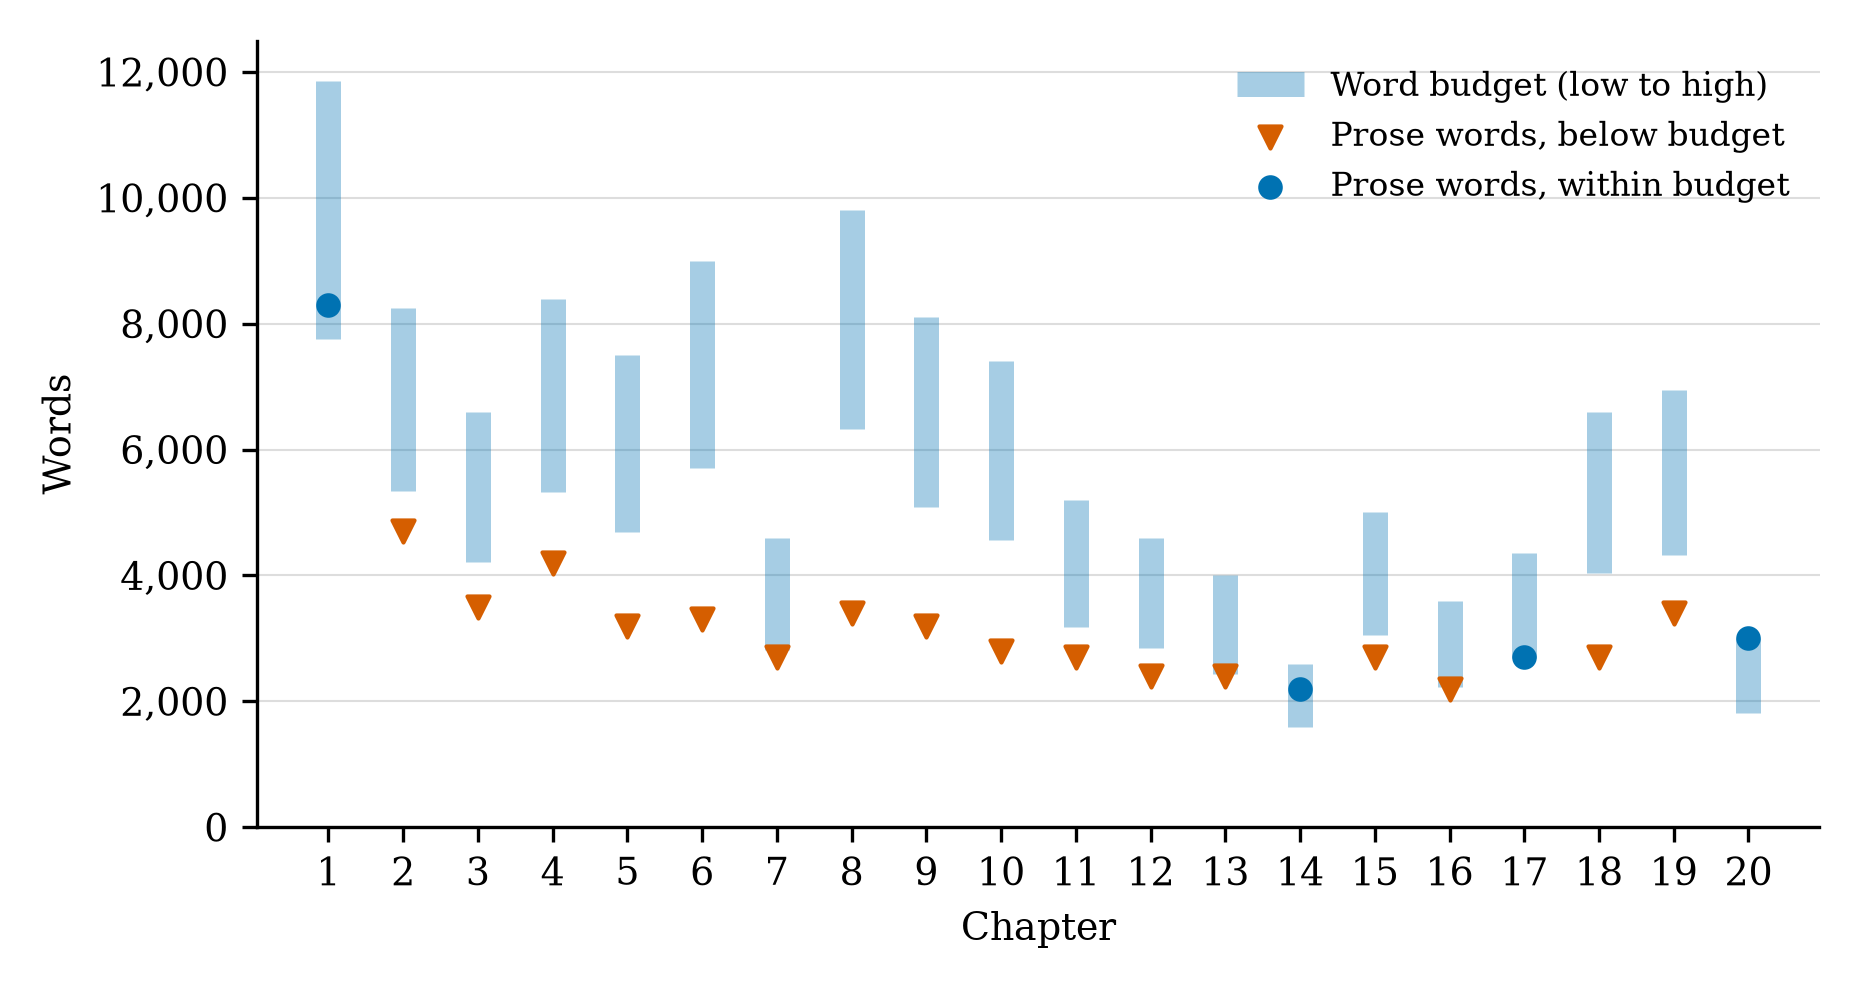
\includegraphics[width=0.85\textwidth]{figures/chapter-budgets.png}
  \caption{Word budget and written prose for the 20 chapters of Case~B, from the chapter
  generator's session log. Bars span each chapter's budget; markers show the prose
  written, excluding simulation specifications and code. Sixteen chapters fall below
  their lower bound. The deviation is a recorded decision, not a hidden one, which is
  what a budget check at the handoff is for.}
  \label{fig:budgets}
\end{figure}

\paragraph{The quiz stage.} The most instructive record is the session log of the quiz
stage, in which the orchestrating agent audited its own run after the author complained
about its speed. A first subagent, assigned all 20 chapters, stopped after seven and
returned an empty report; the orchestrating agent noticed the missing files and launched
a second subagent without establishing why the first had stopped. A command to terminate
a subagent reported success while the subagent kept running. Between polls the
orchestrating agent read finished quizzes and found a wrong answer key, and the strict
build found a broken link anchor. The log then corrects the agent's own earlier claims:
the overall quality score of 82/100 in the published quiz report was hard-coded into the
script that generated the report, the reported distribution of questions across Bloom's
taxonomy levels was assumed rather than measured, and the agent had read parts of only
two of the 20 quizzes and had not reviewed the other 199 questions for
factual correctness. The unsupported score remains in the published report.

\subsection{Case C: an AI-assisted arXiv paper}
\label{sec:case-c}

\paragraph{Context.} The MicroSims paper describes a framework for small AI-generated
educational simulations; it was written by three authors with AI assistance and posted to
arXiv on 25 November 2025 as a 42-page paper with four figures~\cite{lockhart2025microsims}.
Its folder in the project repository contains a main file and eleven section files, a
build script, a status file, a figure-generating script, and a flattened source file and
archive for submission.

\paragraph{Mapping to the framework (RQ1).} The status file is a planning artifact: it
mapped each unfinished section to the documentation chapter it would be condensed from,
with a word count for each source, and estimated about 19,000 words of existing text to
be converted. The abstract, introduction, related work and conclusion were completed
first, while the remaining sections existed as structure with comments marking the content
to be extracted---the planner--executor pattern with the authors as orchestrators. The
build script was the mechanical check, and five intermediate drafts (versions 0.02 to
0.06) were kept, so each revision could be compared with the last. Twenty-three commits
between 17 October and 24 November 2025 record the work; the paper was posted the next
day.

\paragraph{The claim gate.} The draft's ninth section was titled \textit{Empirical
Evidence for Effectiveness}, but the evidence it summarized came from prior studies of
interactive simulations in general, not from measurements of MicroSims. On 18 October
2025 the authors retitled it \textit{Expected Benefits, Limitations and Examples of
Intelligent Textbook Integration}, the title it carries in the posted version, where the
caption of its effectiveness chart names the five studies its values come from. The posted abstract attributes its ``up to 30--40\%'' improvement in
conceptual understanding to physics-education studies and meta-analyses, which makes it a
cited figure, not a measurement of MicroSims. The decision about how to label each
number was made by the authors, which is the human claim gate (I3) at work. The textbook
uses this case to recommend labeling every number in a draft as measured, cited or
expected~\cite{mccreary2026aiforee}.

\subsection{Cross-case analysis}
\label{sec:cross-case}

Table~\ref{tab:defects} lists the 13 defects recorded across Cases~B and~C, coded as
described in Section~\ref{sec:method}.

\begin{table}[htbp]
  \centering
  \caption{Defects recorded in Cases~B and~C, with the failure mode, the control that
  detected each, and the type of that control. ``Agent'' means an execution or
  orchestrating agent noticed the defect; ``self-report'' means agents listed it as an
  open item for the author.}
  \label{tab:defects}
  \footnotesize
  \begin{tabular}{L{0.6cm}L{1.5cm}L{4.8cm}L{2.3cm}L{2.7cm}L{1.9cm}}
    \toprule
    ID & Case, stage & Defect & Failure mode & Detected by & Type \\
    \midrule
    D1 & B, chapters & An acceptance criterion said 2 least significant bits (LSB) of added noise lower ENOB by 1.0--1.5 bits; the drop is about 2.8 bits & Hallucinated result & Hand calculation & Independent calculation \\
    D2 & B, chapters & Stray closing tags after note blocks; the site still built & Malformed output & Tag-counting script & Mechanical \\
    D3 & B, chapters & 16 of 20 chapters below their word budget & Deviation from specification & Budget comparison in log & Mechanical \\
    D4 & B, sims & A specification's rule order gave a different answer than the one intended & Specification error & Built sim checked against specification & Agent \\
    D5 & B, sims & The correct choice was the same at all five steps of a stepper & Specification error & Built sim checked against specification & Agent \\
    D6 & B, sims & Agents wrote content the specifications did not supply & Scope drift & Open-items list & Self-report \\
    D7 & B, sims & A specification revealed answers to later questions & Specification error & Open-items list & Self-report \\
    D8 & B, quizzes & Wrong answer key in one question & Wrong content & Orchestrating agent read a sample & Agent \\
    D9 & B, quizzes & Broken link anchor & Wrong arguments & Strict build & Mechanical \\
    D10 & B, quizzes & Subagent stopped after 7 of 20 chapters with an empty report & Premature completion & Orchestrating agent saw missing files & Agent \\
    D11 & B, quizzes & Termination reported success; subagent kept running & Runaway process & Observed; no control & None \\
    D12 & B, quizzes & Quality score and Bloom distribution hard-coded into a published report & Hallucinated result & Not detected; disclosed in later self-audit & None \\
    D13 & C, manuscript & Section titled as empirical evidence reported other studies' results & Unlabeled claim type & Authors' review; section retitled & Human gate \\
    \bottomrule
  \end{tabular}
\end{table}

D1 shows why the known-answer habit of Case~A matters. Adding Gaussian noise of standard
deviation $\sigma$ to an ideal quantizer with step $\Delta$ (one LSB) raises the noise power from
$\Delta^2/12$ to $\Delta^2/12+\sigma^2$, so with Equation~\eqref{eq:enob} the loss is
\begin{equation}
  \Delta\mathrm{ENOB} = \tfrac{1}{2}\log_2\!\left(1+\frac{12\,\sigma^2}{\Delta^2}\right),
  \label{eq:enob-drop}
\end{equation}
which for $\sigma=2\Delta$ gives $\tfrac12\log_2 49\approx2.81$ bits. The plausible
figure of 1.0--1.5 bits failed a calculation that takes one line.

Three findings answer the research questions.

\paragraph{F1: The framework's elements were present, except the budget (RQ1).} Case~B
used single-purpose roles, files as handoffs, mechanical checks at every handoff and a
status that agents could not set to its final value; Case~C used a planning file, a build
check and a human claim gate. Neither recorded a review budget or measured review time,
and neither had a rule for the provenance of reported numbers.

\paragraph{F2: Each kind of control caught its kind of defect (RQ2).} Mechanical checks
caught every defect for which one existed (D2, D3, D9). Errors of meaning---a wrong
number, a wrong answer key, a mislabeled claim---were caught only when someone recomputed
or read the work: an independent calculation (D1), an agent reading a sample (D8), or the
authors (D13). Three specification errors (D4, D5, D7)
surfaced when execution agents tried to build what a planning agent had specified: the
planner--executor handoff acted as a check on the plan, which is the benefit of reviewing
plans before execution~\cite{shen2023hugginggpt,schluntz2024building}, obtained here
without the researcher. Two defects (D6, D7) were reported by the agents themselves but
await the author's review, because the human gate had not yet been reached.

\paragraph{F3: The escaped defects violated the invariants and lacked a mechanical
defense (RQ3).} D12 escaped every control. The agent that orchestrated the quiz stage
also produced and published the quality score of that stage's output, which is a breach
of separation of acceptance (I1), and the score came from no computation, which no check in the original
framework could detect. The provenance rule P of Section~\ref{sec:handoff} closes that
gap: a script that requires every reported number to name the call that produced it
would have rejected the report. D10 and D11 were caught, when they were, only because the
orchestrating agent happened to notice. Both argue for the defense listed against
premature completion in Table~\ref{tab:failures}---check output in every handoff---and for
process-level limits enforced by the harness rather than by the agent. Finally, the
timing gaps in Case~B show that logs narrated by an agent are not a reliable instrument:
the review-load parameters of Equation~\eqref{eq:load} can only be measured if the harness
writes the timestamps.

\section{Discussion}
\label{sec:discussion}

The cases support the paper's central claim in a specific form. Where a mechanical check
existed it worked, and where the plan was handed to a separate executor the handoff
exposed errors in the plan. What failed was what the original framework left implicit:
nobody recorded the reviewer's time, and nothing tied a reported number to the
computation that should have produced it. Both gaps concern the researcher's attention,
which is the quantity the framework puts at the center.

\subsection{Implications}
\label{sec:implications}

\paragraph{For researchers.} The assignment rule turns a vague question---how much should
I trust this agent?---into three questions about the task that can be answered before
any agent runs. Its monotonicity suggests the cheapest route to more delegation: change
the task rather than the model, by writing outputs to new files, adding a known-answer
test or keeping results local until they are accepted. Before a team is enlarged, the
review load $L$ and the number of defects found after acceptance $E$ should be measured on
a small pilot, because Equation~\eqref{eq:escape} shows that reading less is paid for in
escaped defects unless mechanical checks take up the difference. The source textbook
orders adoption accordingly: a group policy and a repository with an instruction file
come first, then one skill piloted at level 1 or 2, then checks and a reproducibility
package, and only then a small team, reviewed after 90 days on time saved, review time
and errors that escaped~\cite{mccreary2026aiforee}.

\paragraph{For advisors and research groups.} Most of the framework is a set of
conventions that a group can share: an instruction file, a vocabulary of statuses with
\textsf{accepted} reserved for people, a template for handoff records and a short record
of each acceptance before a result enters a paper. Case~B shows a side benefit: a status
field that agents cannot advance makes the review backlog visible, here as 50 simulations
awaiting approval. A backlog that is visible can be managed; one hidden in agents'
reports cannot. Because reviewers tend to accept automated output with less scrutiny
over time~\cite{parasuraman2010complacency,goddard2012automation}, a group can also ask
reviewers to state the expected value before reading an artifact or to check a random
sample rather than the first few items.

\paragraph{For builders of agent tools.} Four of the case findings point to features
of the harness rather than of the model. The harness, not the agent, should write
timestamps and record how long each artifact waited for and received review, so that
$k_j$, $r_j$ and $s_j$ can be measured. It should make \textsf{accepted} impossible for the
producing agent to set (I1). It should enforce step, time and spending limits and confirm
that a terminated process has stopped, which D11 shows an agent cannot be trusted to
report. And it should support the provenance rule by linking each number in a report to
the call that produced it, in the spirit of activity logging for
agents~\cite{chan2024visibility}.

\paragraph{For venues.} Current policies ask authors to disclose substantial use of
generative AI and to take responsibility for the
result~\cite{arxiv2025genai,nature2023tools,ec2025living}. A disclosure that named which
tasks were delegated, at which autonomy level, and which claims passed a human gate would
tell reviewers more than a statement that a tool was used. This is a suggestion that
follows from the framework, not a finding of this study.

\subsection{Limitations}
\label{sec:limitations}

\begin{enumerate}[leftmargin=*]
  \item \textit{Author bias.} The framework, the textbook it comes from and both real
    cases are the author's own, and one person coded the defects. An independent coder
    might classify some defects differently, particularly the boundary between agent
    checks and self-reports.
  \item \textit{Case selection.} Cases~B and~C are publication pipelines---a textbook and
    a paper---not laboratory research with instruments. The engineering case is
    illustrative. That the framework transfers to measurement-heavy research is argued
    from its structure, not shown.
  \item \textit{Unmeasured parameters.} Review times, the attention budget, the
    planning-to-execution ratio and the detection probabilities in
    Equations~\eqref{eq:load}--\eqref{eq:pipeline} are illustrative. The model's
    predictions, such as the span of control, have not been tested against observed
    teams.
  \item \textit{Binary task properties.} In practice reversibility, reach and
    verifiability are matters of degree: an action can be partly reversible, and a check
    can be cheap for one reviewer and expensive for another. The rule is a first cut that
    graded or probabilistic versions could refine.
  \item \textit{Incomplete records.} The logs were partly narrated by the agents
    themselves, timestamps were missing, and one log contained a number that no
    computation produced. Defects that were never recorded cannot be counted, so the 13
    defects are a lower bound, not a rate.
  \item \textit{One orchestrator.} The model assumes a single researcher. Groups with
    several reviewers, delegated review and shared queues raise coordination questions it
    does not address.
  \item \textit{Pace of change.} Agent products and models change within months. The
    framework is stated without reference to any product, but the parameter values that
    make it useful will drift and must be re-measured.
\end{enumerate}

\section{Conclusion and Future Work}
\label{sec:conclusion}

Agents can now perform much of the procedural work of engineering research, but they
cannot carry its accountability, and the researcher who does carry it has a fixed number
of hours in which to check what the agents produce. This paper turned that observation
into a working framework. Autonomy is granted per task from what the task can do to the
world---whether its result escapes, whether it can be undone, whether it can be
checked---and the rule that does so never penalizes making a task safer. Work moves as
files whose acceptance belongs to someone other than their producer, and numbers must
show where they came from. Team size is set by the review budget, from which the
familiar two-to-one ratio of planners to executors falls out as a consequence of review
costs. Applied to an illustrative converter characterization and to two real
publication projects, the framework's controls matched where the recorded defects were caught,
and the one defect that reached publication unchecked fell exactly where the original
framework had no control.

Five directions would turn the framework's illustrative parameters into measured ones.
\begin{enumerate}[leftmargin=*]
  \item \textit{Measure review load in a working group.} Instrument an agent harness to
    record, for each artifact, its producer, its waiting time, the reviewer's time and the
    acceptance decision, over a semester in a research group; estimate $k_j$, $r_j$, $s_j$
    and $E$, and test whether the span of control of Equation~\eqref{eq:span} predicts the
    observed review backlog.
  \item \textit{Test the reliability of the assignment rule.} Ask several engineering
    researchers to code the same set of tasks for reach, reversibility and verifiability
    independently, report inter-rater agreement, and replace binary properties with graded
    ones where agreement is low.
  \item \textit{Implement the provenance rule as a validator.} Build a check that rejects
    any agent report containing a number without a producing call, and evaluate it on
    reports with seeded defects of the kind of D12.
  \item \textit{Apply the framework to physical measurement.} Run the characterization of
    Case~A on a real converter, with test methods from the ADC test
    standard~\cite{ieee1241}, and compare escaped defects with and without the claim gate.
  \item \textit{Represent handoffs as a knowledge graph.} Store tasks, artifacts, checks
    and acceptances as linked entities, so that a query can list every claim that depends
    on an artifact later found to be wrong, building on work on personal knowledge
    graphs~\cite{mccreary2023pkg}.
\end{enumerate}


\section*{Acknowledgments}
The MicroSims case study in Section~\ref{sec:case-c} draws on a paper the author wrote
with Valerie Lockhart and Troy A. Peterson. The textbook case study in
Section~\ref{sec:case-b} uses the public repository of the book and its session logs.

\paragraph{Use of generative AI.}
Generative AI was used in two ways, and both are reported here. First, the textbook and
the MicroSims paper studied in Section~\ref{sec:cases} were produced with AI agents, as
those sections describe. Second, this paper was drafted with Claude Opus 5.5 (Anthropic),
running in Claude Code with an agent skill for arXiv paper preparation. The model
condensed the author's textbook and project records into the sections, wrote the figure
scripts and TikZ diagrams, and retrieved and formatted bibliographic metadata; every
reference was checked against Crossref, DataCite, or the publisher's page. The author
reviewed, edited and verified all content, including every citation and every number
drawn from the project logs, and takes full responsibility for this paper.

% References
\bibliographystyle{ieeetr}
\bibliography{sections/references}

\end{document}
